
%(BEGIN_QUESTION)
% Copyright 2015, Tony R. Kuphaldt, released under the Creative Commons Attribution License (v 1.0)
% This means you may do almost anything with this work of mine, so long as you give me proper credit

\noindent
{\bf Demonstration Program -- counter instructions} 

\vskip 10pt

An important technique for learning any programming language -- Ladder Diagram PLC programming included -- is to write simple ``demonstration'' programs showcasing and explaining how particular instructions and programming constructs are supposed to work.  Since you have access to your own personal PLC, you can explore the elements of your PLC's programming language like a scientist would explore new specimens: subject them to tests and record how they respond.  This is how you will be able to teach yourself new models of PLC when you are working in your career, when you won't have textbooks to follow or training to show you exactly what to do.

\vskip 10pt

Write such a ``demonstration'' program for your PLC's {\it counter} instructions, where discrete inputs on your PLC control discrete outputs on your PLC.  An acceptable demonstration program must meet these three criteria:

\begin{itemize}
\item{} {\bf Simple} -- nothing ``extra'' included in the program to detract from the fundamental behavior of the instruction(s) being explored
\vskip 5pt
\item{} {\bf Complete} -- nothing missing from the program relevant to the fundamental behavior of the instruction(s) being explored.  {\it For a counter demonstration program, this includes up counters, down counters, and up/down counters, all with provision for re-setting.}
\vskip 5pt
\item{} {\bf Clearly documented} -- every rung clearly commented in your own words, every variable named
\end{itemize}

{\it Your instructor will challenge you to use this demonstration program to illustrate what you have learned about PLC counter instructions.}


\vskip 20pt \vbox{\hrule \hbox{\strut \vrule{} {\bf Suggested questions your demonstration program should answer:} \vrule} \hrule}

\begin{itemize}
\item{} What are the different counter instruction types offered on your PLC?  What does each one of them do?
\item{} How can you make a single counter both {\it increment} (count up) and {\it decrement} (count down)?
\item{} Where in the PLC programming editor can you view the ``live'' status of a counter instruction?
\item{} Where in the PLC's memory are the counter variables (e.g. accumulated value, setpoint value) located?  What symbol(s) are used to address each one?
\item{} How far up can a counter count?  How far down?  Note that this will be related to the number of bits the counter instruction uses to track its current (accumulated) value.
\item{} What happens when a counter reaches its preset value?  How do you use this event to trigger something else to happen in the program?
\item{} What happens to the counter's current value when it reaches its preset value?  Does the counter stop counting, or does it continue counting past this threshold?
\item{} When a counter is reset, does its current value begin at zero or one?
\item{} Is it possible to ``preload'' a counter instruction so that it doesn't have to begin at the starting value when the PLC program runs anew?
\item{} What happens to the counter's current value when it reaches its maximum value?  Does the counter instruction stop counting, or does it do something else?
\end{itemize}

\underbar{file i03353}
%(END_QUESTION)





%(BEGIN_ANSWER)

There are no answers provided here!  For help, consult the ``instruction set'' reference manual for your PLC, which will describe in detail how each type of instruction is supposed to function in your PLC.
 
%(END_ANSWER)





%(BEGIN_NOTES)

\noindent
{\bf Summary Quiz:}

The recommended summary quiz is to have \underbar{each student} demonstrate their PLCs running this demonstration program.  Demonstration programs should not be accepted unless and until they meet all three criteria listed in the question: they need to be {\it simple} (no extraneous features), {\it complete} (demonstrating {\it all} the necessary instructions), and {\it thoroughly documented} in the student's own words (every rung commented intelligently, every variable named).

\vskip 10pt

Some students may opt to write separate demonstration programs for each type of counter instruction supported by their PLC.  This is a perfectly acceptable alternative to writing a single demonstration program showcasing all counter instruction types.

\vskip 10pt

When checking students' demonstation programs, have them run the programs with their laptop PCs in online mode so they can view status highlighting and numerical values live, and {\it ask them to provide a running commentary of what they see the instructions doing.  If their commentary is lacking, challenge them to explore instruction behaviors that they have not yet done.}  Refer to the ``suggested questions'' for specific ideas on instruction behavior that may be explored in a demonstration program.

\vskip 10pt

This is by far the most important PLC program students will write today.  If there are other programs assigned in this day's plan, {\it prioritize this one}.  This point bears mentioning because a common error students make is to disregard the importance of a well-written demo program, instead tending to treat it as ``busywork'' and move on to ``more important'' assignments.  As the instructor your task is to explain why demonstration programs are important and to ensure students take them seriously:

\begin{itemize}
\item{} Demonstration programs are a powerful tool for self-instruction later when graduates will be challenged to learn some new PLC system.
\vskip 5pt
\item{} Demonstration programs may be re-run at a later date, which makes them ideal tools for review near the conclusion of the course.
\vskip 5pt
\item{} Demonstration programs require students to scientifically observe the PLC's programmed behavior, learning by {\it experiment} rather than learning by {\it direct instruction}.
\vskip 5pt
\item{} Well-written comments demand critical reflection on the part of the student, and also serve as practice for technical expression.
\end{itemize}









\vfil \eject

\noindent
{\bf Sample demonstration program for up and down counter instructions:} (for an Allen-Bradley MicroLogix PLC)

$$\epsfysize=6in \includegraphics[width=15.5cm]{i03353x01.eps}$$

%INDEX% PLC, demonstration program: counter instructions

%(END_NOTES)


